\documentclass[uplatex,dvipdfmx,a4paper,twocolumn,base=11pt,jbase=11pt,ja=standard]{bxjsarticle}  % 環境に合わせて変更してください

\usepackage{ipsj}
\usepackage{color}
\usepackage{enumerate}
\usepackage{url}
\usepackage[dvipdfmx]{graphicx}
\usepackage{caption}

\newcommand{\todo}[1]{\colorbox{yellow}{{\bf TODO}:}{\color{red} {\textbf{[#1]}}}}

\title{直観的なScratch作品のためのユーザ入力タイミング特定の試み}{Toward identifying user input timing for intuitive Scratch work search}
\author{和歌山大学}{岡本 圭悟}{Keigo Okamoto, Wakayama University}
\author{和歌山大学}{伊原 彰紀}{Akinori Ihara, Wakayama University}
\author{和歌山大学}{三倉 舞子}{Maiko Mikura, Wakayama University}
\author{和歌山大学}{橋谷 直樹}{Naoki Hashitani, Wakayama University}

\begin{document}
\maketitle

%================
%1
\section{はじめに}
%================

ビジュアルプログラミング言語の学習環境の一つであるScratch\footnote{\url{Scratch: https://scratch.mit.edu/}}では,膨大な作品が公開されている.ユーザは多様な実装方法を参照するために,作品をキーワード検索によって絞り込むことができる.しかし,ユーザが実装する動作イメージを言語化することは容易でないため,そのイメージに類似する作品の検索は困難である.
従来研究\cite{thesis_fukuchi2021}では,ユーザがイメージするオブジェクトの移動軌跡をマウス操作によって入力し,それをクエリとする作品検索を実現しているが,検索にはあらかじめ作品を自動実行してスナップショットを撮影する必要があるため,入力操作を持つ作品は対象にできない.

本研究の事前分析ではScratchの入力操作を持つ作品数,および実装に必要な計算論理的思考能力をDr.Scratch~\cite{RED2015_J. Moreno-Le ́on}を用いて定量的に計測した.Scratchの入力操作を持つ作品は,入力操作を持たない作品の10倍以上存在する.また,図\ref{fig:score}は入力操作を持つ作品と入力操作を持たない作品の実装に必要な計算論理的思考を0点から21点までの値で定量化した分布を示す.,入力操作を有する作品は,入力操作を持たない作品に比べて計算論理的思考の熟練が必要であり,マンホイットニーのU検定を用いて統計的有意差(p値$<$0.01)を確認した.従って,
%データ間に有意差があることも示された.このことから,入力操作を持つ作品はより多様な命令処理を必要とすることは明らかである.したがって,
入力操作を有する作品を検索の対象に含むべきであるが,入力のタイミングをオブジェクトの移動軌跡のみから判断することは容易でない.

本研究は,入力を有する作品検索の実現に向けて,作品中でユーザが入力操作するタイミングを特定し,自動実行するシステムを提案する.具体的には,Scratchプログラムから,入力前後の命令処理,入力内容,入力前後のオブジェクトの位置を収集し,ユーザが入力操作するタイミングを特定する.

\begin{figure}
    \begin{center}
        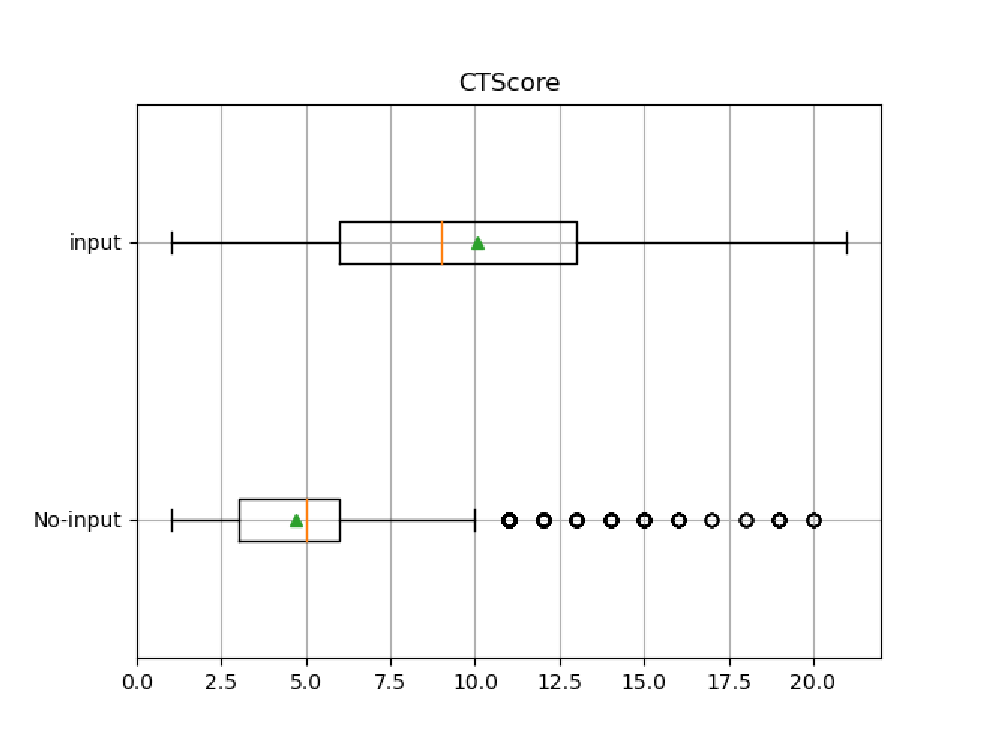
\includegraphics[width=0.\linewidth]{plot.eps}
        \caption{入力操作をもつ作品と持たない作品のCTスコアの分布}
        \label{fig:score}
    \end{center}
\vspace{-10mm}
\end{figure}


%================
%2.2
\section{提案手法}
%================
本研究で検索対象に新たに含む作品の条件を示し,作品中においてユーザが入力操作するタイミングを特定,および入力操作を自動化する手順を述べる.%は,Scratch上で公開されている作品から,以下に示す条件を満たす作品を用いる.
\begin{itemize}
 \item \todo{XX}のため,ユーザの操作を有するブロックのうち,文字の入力でないキー入力のみを有するブロックを含む作品
 \item \todo{XX}のため,ユーザの定義した変数や関数を含まない作品
 \item \todo{XX}のため,座標移動を行うブロックを含む作品
\end{itemize}

\noindent\textbf{1. ブロック情報の取得: }\todo{事前にScratch APIによって取得した作品のプログラム情報(sbiファイル?)を解析し,}対象のScratch作品に含まれる座標ブロック,ユーザの操作を有するブロックの種類,およびブロックの実行順序を取得する.\\
\noindent\textbf{2. 座標の計算: }\todo{「入力操作が発生するタイミング,および入力操作によりオブジェクトの移動場所を特定するため?」},Scratch作品のプログラム実行よりオブジェクトの移動元,移動先の座標を計算する.\\
%作品が実行されてからユーザの操作を有するブロックが処理されるまでにオブジェクトが到達する座標をプログラム上で計算する.\\
\noindent\textbf{3. 入力タイミングの決定: }ブラウザ操作を自動化するSeleniumを用いて,入力操作が発生するタイミングにキー入力を実行する.作品のスクリプトの処理が終了するまで,または作品のスクリーンショットの撮影時間が終了するまで繰り返す.

%座標に画像オブジェクトが到達したときを入力すべきタイミングとして,自動でキーを押下する.これをスクリプトが処理を終了するまで繰り返す.

「ループブロック」などの制御ブロック中に処理終了をスクリプトの処理の終了とする.\todo{←よくわからん}また,並列にスクリプトが存在する場合も同様の手順でスナップショットを撮影する.

%================
%2.4
\section{ケーススタディ}
%================

Scratchにおいて公開される作品の中から\todo{入力操作を有する?作品を}ランダムに10件抽出し,本手法で撮影したスナップショットを確認する.その結果,10件中9件の作品に対して入力のタイミングを自動特定することができた.入力のタイミングを取得できなかった作品\footnote{\url{http://hogehoge}}のプログラムを図\ref{fig:input}に示す.この作品では,スペースキーの後に上矢印キーのように順に入力すべきである.しかし,提案手法では座標移動の情報のみで入力のタイミングを特定しているため,入力ブロック間に座標移動ブロックが存在しないようなプログラムでは入力のタイミングを特定できない.今後は,\todo{解決方法があれば描きたい}

\begin{figure}
    \begin{center}
        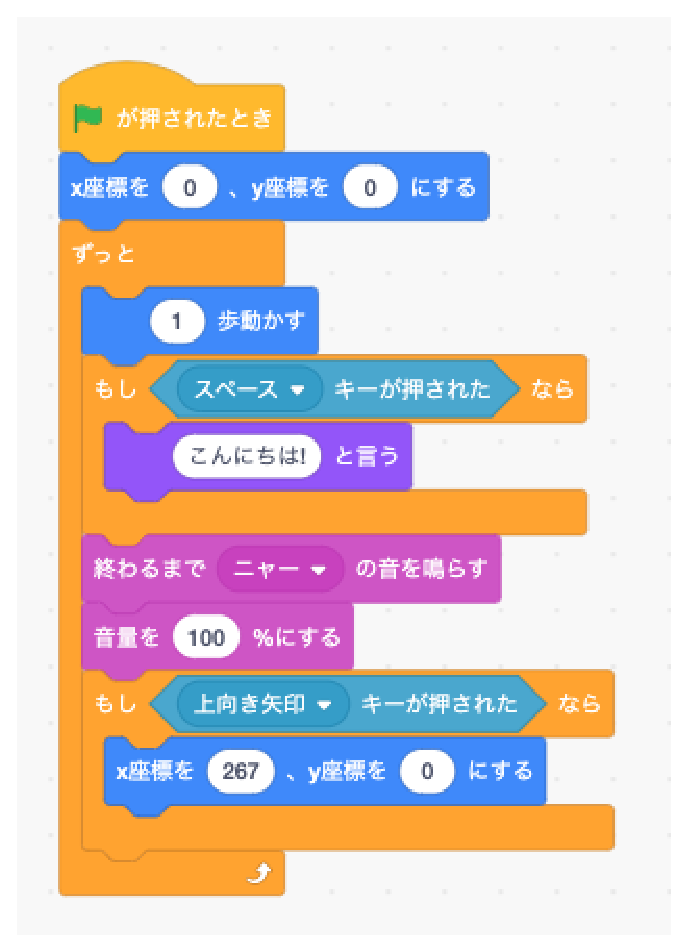
\includegraphics[width=0.5\linewidth]{program.eps}
        \caption{入力タイミングを取得できなかったプログラム}
        \label{fig:input}
    \end{center}
\vspace{-8mm}
\end{figure}

%
%\subsection{動作実験}
%================

%提案手法を用いてデータセット に含まれる作品20件を実行したところ,全ての作品において入力のタイミングを特定して自動で入力操作を行うことが確認できた.

%================
%3
\section{おわりに}
%================

本論文では,入力を有する作品を含んだ学習者の動作イメージと類似する作品検索に向けて.自動で入力操作を行うタイミングの特定を試みた.今後は,本手法を用いて撮影したスナップショットを用いて検索候補を増加し,検索結果の多様性の向上を目指す.



\begin{thebibliography}{1}
  \bibitem{thesis_fukuchi2021} 福地ユキ,伊原彰紀,山本豪志朗,橋谷直樹,ビジュアルプログラミング作品検索のためのオブジェクト操作データの時系列解析,情報処理学会関西支部, 2021
  \bibitem{RED2015_J. Moreno-Le ́on} J. Moreno-Le'on, G. Robles, and M. Rom'an-Gonz'alez, ``Dr. scratch: Automatic analysis of scratch projects to assess and foster computational thinking,'' RED.Revista de Educaci'on a Distancia, vol.15, no.46, pp.1-23, 2015.
  \bibitem{ICMSR2017_Aivaloglou} E. Aivaloglou, F. Hermans, J. Moreno-Le'on, Gr. Robles, ``A dataset of scratch programs: scraped, shaped and scored,'' Proceeding of the International Conference on Mining Software Repositories (MSR'17), pp.511-514, 2017. 

\end{thebibliography}




\bibliographystyle{ipsjunsrt}
%\bibliography{bibfile}

\end{document}
